\section{Budget}
\subsection{Component Selection}
\subsubsection{Button Triggers}
To accurately observe the approximately-linear motion of a piano key, we feel a linear push-button switch is our best choice. We do not want any sort of locking mechanism because the key should be registered as ‘on’ when pressed and ‘off’ when released and each key will need two switches, which is a total of sixty-four total switches in the keyboard keys alone. Linear push-button switches provide this linear on-off response and come with a low price tag.

Since we want our project to feel as close to a professional MIDI controller as possible, we do not want our user to know there is a button being actuated separately from the key. This means our buttons should be almost silent and not provide any tactical feedback. To achieve these parameters we did our research and brought three types of buttons to debate: the Odseven Soft Tactile Button, the Panasonic ESE-20d443, and the Nidec Copal TR1-01. These three choices offered are a single-pole single-throw linear push-button with a silicon cover. Their images and data are shown in Figure \ref{fig:buttons_fig} and Table \ref{Tab:buttons_data} .

\begin{figure}[h!]
  \centering
  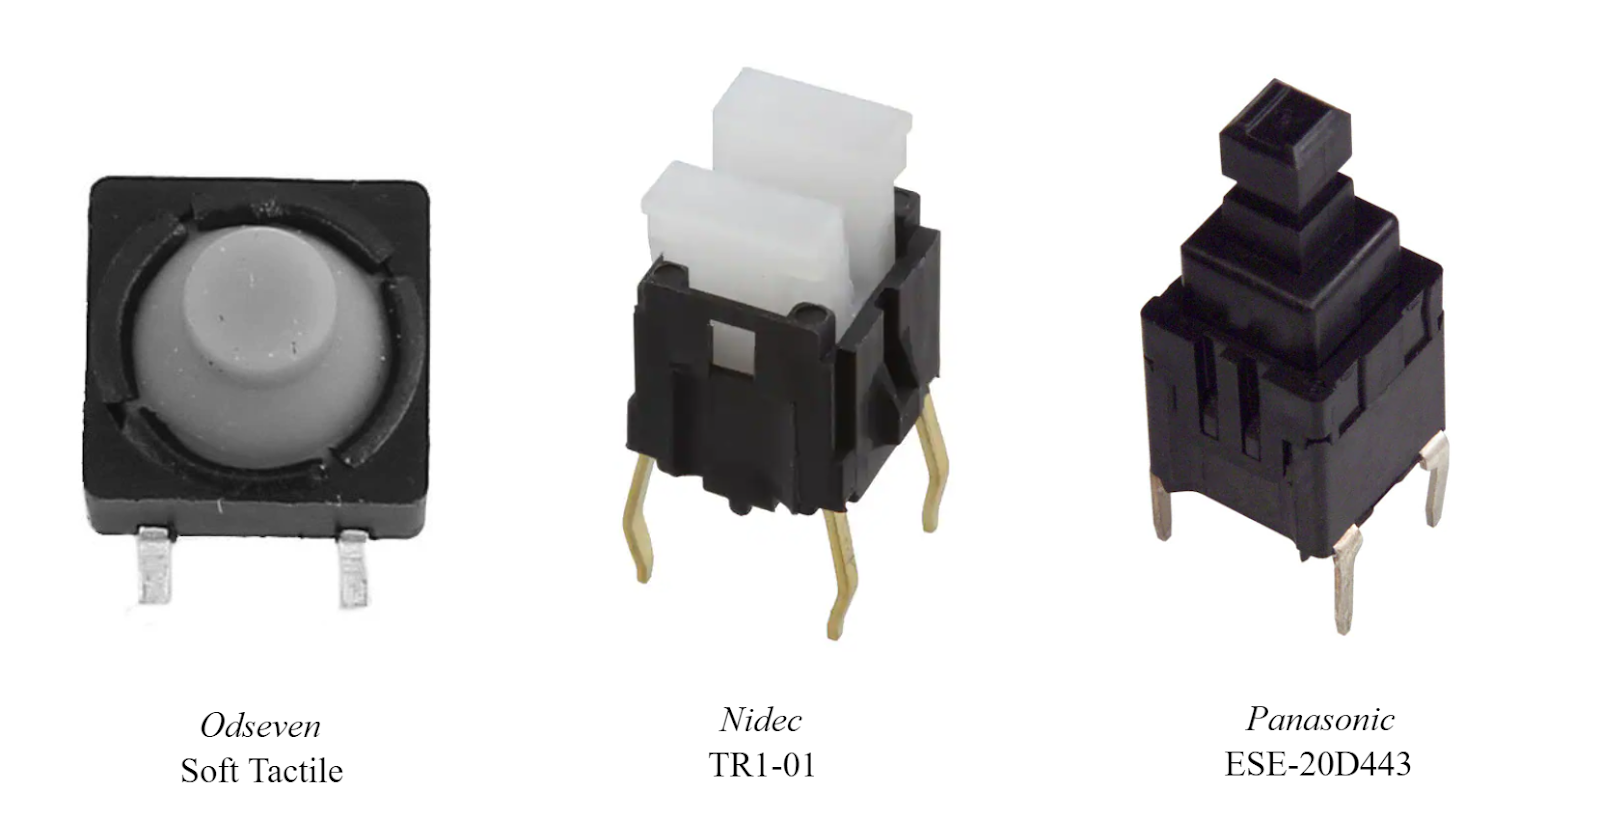
\includegraphics[width=\linewidth]{image/Buttons.png}
  \caption{A comparison of button options}
  \label{fig:buttons_fig}
\end{figure}

\begin{table}[h!]
  \centering
  \resizebox{\textwidth}{!}{%
  \begin{tabular}{|l|l|l|l|}
    \hline
    Brand                           & Cost   & Quantity & Form Factor               \\ \hline
    Odseven                         & \$1.17 & 10       & 7.8mm x 7.8mm x 4.9mm     \\ \hline
    Nidec Copal Electronics         & \$0.54 & 1        & 5.9 mm x 7 mm x 9 mm      \\ \hline
    Panasonic Electronic Components & \$1.31 & 1        & 7.9 mm x 7.8 mm x 17.5 mm \\ \hline
  \end{tabular}}
  \caption{}
  \label{Tab:buttons_data}
\end{table}

After debating which option would be the best for this project, we ultimately settled on the Odseven Soft Tactile button for a few reasons. First, as we can see in Figure \ref{fig:buttons_fig} and the accompanying Table \ref{Tab:buttons_data}, The Nidec and the Panasonic buttons extend at least twice as high as the Odseven. Although the taller buttons could provide more constant contact with the key and reduce the feeling of multiple actuations, the button would need to be in actual constant contact during the entire actuation to make a difference in feel. On top of that, to receive information for velocity, we would need to place the buttons in different locations on the key and have different actuation distances from the key for each button. No matter our choice, constant contact would require two different types of buttons. Plus, the total actuation of the key is five degrees and we would need to find two buttons with extremely precise height and actuating distance.

The next reason we chose the Odseven Tactile Soft button was because of the shape of the button itself. With a circular head and smallest actuation distance, it appears to be more versatile for our multistage actuation set-up, where the key is pressed before it presses the button itself. We could use a variety of rod shapes connected to the key and still get the Odseven button to actuate properly. This will come in handy during the prototyping and reiteration of the project. Additionally, the datasheets provided with these devices do not offer a decibel reading of the button response. The only button which discussed sound was the Odseven which claims to be “silent”. From our experience as musicians, we would much rather take a key that has an odd feeling when pressed over a key that clicks when pressed.

The final reason we chose the Odseven button is the price. We have a budget goal of below five-hundred dollars and Odseven sells this button, as well as Adafruit, at a significantly lower price per button than the other options. Our project will be using sixty-four buttons in the keys alone and every unnecessary dollar spent on buttons will add up quickly.

\begin{table}[h!]
  \centering
  \resizebox{\textwidth}{!}{%
  \begin{tabular}{|l|l|l|l|l|}
    \hline
    \textbf{Item}                                 & \textbf{Cost}   & \textbf{Quantity}   & \textbf{Total}   & \textbf{Notes}                                                        \\ \hline
    Batteries                                     & \$7             & 2                   & \$14             & We do not know power requirements                                     \\ \hline
    Microcontroller / CPU                         & \$45            & 1                   & \$45             & We do not know computational requirements                             \\ \hline
    Mechanical Springs                            & \$1.50          & 24                  & \$36             &                                                                       \\ \hline
    Reels of 3D Filament                          & \$15            & 2                   & \$30             &                                                                       \\ \hline
    6.35 mm Audio Jack                            & \$2.50          & 1                   & \$2.50           &                                                                       \\ \hline
    USB-B Output                                  & \$2             & 1                   & \$2              & CPU (such as Pi) may have this already                                \\ \hline
    Power Input                                   & \$2.50          & 1                   & \$2.50           & CPU (such as Pi) may have this already                                \\ \hline
    Key buttons                                   & \$0.50          & 48                  & \$24             &                                                                       \\ \hline
    Click Knob                                    & \$2             & 2                   & \$4              &                                                                       \\ \hline
    12v to 5v Step Down                           & \$5             & 1                   & \$5              &                                                                       \\ \hline
    UI Buttons                                    & \$10            & 1                   & \$10             &                                                                       \\ \hline
    720p Display                                  & \$25            & 1                   & \$25             &                                                                       \\ \hline
    Charging Circuit                              & \$5             & 1                   & \$5              &                                                                       \\ \hline
    Acrylic Screen Protection                     & \$10            & 1                   & \$10             &                                                                       \\ \hline
    Electrical Wiring Rolls                       & \$15            & 1                   & \$15             &                                                                       \\ \hline
    Laser cut / CNC wood                          & \$40            & 1                   & \$40             & No clue on the price considering we haven't fully discussed options   \\ \hline
    \textbf{Total cost before tax and shipping }  &                 &                     & \textbf{\$270 }  &                                                                       \\ \hline
  \end{tabular}}
  \caption{Proposed budget}
  \label{Tab:budget}
\end{table}
